\documentclass[10pt,conference]{IEEEtran}
\IEEEoverridecommandlockouts
\usepackage[T1]{fontenc}
\usepackage{cite}
\usepackage{amsmath,amssymb}
\usepackage{graphicx}
\usepackage{booktabs}
\usepackage{array}
\usepackage{xcolor}
\usepackage{url}
\usepackage{balance}
\usepackage{pgfplots}
% Shipped with compat=1.18 (current pgfplots). The local build machine has TeX Live 2020 (pgfplots 1.17),
% where 1.18 is fatal; `make pdf` in ../artifact seds this to 1.17 in a build copy.
\pgfplotsset{compat=1.18}
\usetikzlibrary{shapes.callouts,arrows.meta}
\usepackage[ruled,linesnumbered,noend]{algorithm2e}
\SetAlFnt{\footnotesize}
% generated by artifact/src/render.py -- do not edit
\newcommand{\BpBDecided}{1}
\newcommand{\BpBDecidedHi}{3}
\newcommand{\BpBDecidedLo}{0}
\newcommand{\CpeCoder}{7.0}
\newcommand{\CpeGeneral}{6.7}
\newcommand{\CpeHaiku}{9.2}
\newcommand{\DbpDecided}{24}
\newcommand{\DbpDecidedHi}{30}
\newcommand{\DbpDecidedLo}{18}
\newcommand{\DecTrueShare}{99.7}
\newcommand{\ExtAgree}{50}
\newcommand{\ExtAgreeHi}{61}
\newcommand{\ExtAgreeLo}{40}
\newcommand{\ExtFalseFirst}{0.0}
\newcommand{\ExtFalseSecond}{0.0}
\newcommand{\ExtKappa}{0.52}
\newcommand{\ExtMatched}{77}
\newcommand{\ExtN}{30}
\newcommand{\ExtNfunc}{15}
\newcommand{\ExtSdDecidedSecond}{64}
\newcommand{\ExtSecondFalse}{0}
\newcommand{\ExtSecondFalseVfour}{3}
\newcommand{\ExtSecondFalseVfourCorrect}{0}
\newcommand{\FaCorrect}{1}
\newcommand{\FaLocal}{1}
\newcommand{\FaN}{1}
\newcommand{\FaPrevAll}{27}
\newcommand{\FaPrevLocal}{15}
\newcommand{\FathreeAllTrue}{26}
\newcommand{\FathreeCorpusCorrectRefutation}{1}
\newcommand{\FathreeCorpusFactBug}{8}
\newcommand{\FathreeCorpusFactGapSplat}{5}
\newcommand{\FathreeCorpusLocalCorrectRefutation}{1}
\newcommand{\FathreeCorpusLocalFactBug}{5}
\newcommand{\FathreeCorpusLocalFactGapSplat}{5}
\newcommand{\FathreeCorpusLocalMisSlot}{4}
\newcommand{\FathreeCorpusMisSlot}{13}
\newcommand{\FathreeLocalTrue}{14}
\newcommand{\FathreePlantedCorrectRefutation}{1}
\newcommand{\FathreePlantedEngineBugFixedVF}{1}
\newcommand{\FathreePlantedMisSlot}{2}
\newcommand{\FlipCallsIndirectToConsistent}{3}
\newcommand{\FlipFamCallsImports}{3}
\newcommand{\FlipFamFlow}{38}
\newcommand{\FlipFamProbe}{49}
\newcommand{\FlipFamReturns}{30}
\newcommand{\FlipFlowControlToConsistent}{2}
\newcommand{\FlipFlowSelfToUnverifiable}{10}
\newcommand{\FlipFlowUnresolvedToUnverifiable}{26}
\newcommand{\FlipIntoTrue}{15}
\newcommand{\FlipIntoTrueFromFalse}{8}
\newcommand{\FlipIntoTrueFromUndischargeable}{7}
\newcommand{\FlipProbeInstantiatedConsistentToConsistent}{10}
\newcommand{\FlipProbeInstantiatedUnverifiableToUnverifiable}{32}
\newcommand{\FlipProbeNoneUnverifiableToUnverifiable}{7}
\newcommand{\FlipReturnsOtherToUnverifiable}{1}
\newcommand{\FlipReturnsUncheckedToConsistent}{29}
\newcommand{\FlipTotal}{120}
\newcommand{\FlipVoneDecided}{55.2}
\newcommand{\FlipVoneTrue}{420}
\newcommand{\HoneConsistent}{9.0}
\newcommand{\HoneConsistentHi}{11.5}
\newcommand{\HoneConsistentLo}{6.7}
\newcommand{\HoneDecons}{47.4}
\newcommand{\HoneDeconsHi}{52.9}
\newcommand{\HoneDeconsLo}{41.7}
\newcommand{\HoneFull}{38.4}
\newcommand{\HoneFullHi}{43.9}
\newcommand{\HoneFullLo}{32.7}
\newcommand{\HoneFullNoprule}{39.5}
\newcommand{\HoneFullNopruleHi}{45.1}
\newcommand{\HoneFullNopruleLo}{33.8}
\newcommand{\HoneHeld}{38.0}
\newcommand{\HoneHeldHi}{45.2}
\newcommand{\HoneHeldLo}{30.2}
\newcommand{\HoneHeldN}{498}
\newcommand{\HoneHeldNoprule}{38.8}
\newcommand{\HoneHeldNopruleHi}{46.0}
\newcommand{\HoneHeldNopruleLo}{31.2}
\newcommand{\HoneNdisagreeLocal}{9}
\newcommand{\HoneRoundB}{43.5}
\newcommand{\HoneRoundC}{34.4}
\newcommand{\HoneRoundD}{37.8}
\newcommand{\HoneRoundE}{37.9}
\newcommand{\HoneRoundF}{38.2}
\newcommand{\HtwoAgree}{95}
\newcommand{\HtwoCDropped}{732}
\newcommand{\HtwoCHi}{--}
\newcommand{\HtwoCLo}{--}
\newcommand{\HtwoCN}{32}
\newcommand{\HtwoCP}{--}
\newcommand{\HtwoCPperm}{1.000}
\newcommand{\HtwoCRho}{-0.07}
\newcommand{\HtwoCTau}{-0.07}
\newcommand{\HtwoCXone}{31}
\newcommand{\HtwoCYone}{28}
\newcommand{\HtwoEfJf}{0}
\newcommand{\HtwoEfN}{1}
\newcommand{\HtwoJfEf}{0}
\newcommand{\HtwoJfN}{13}
\newcommand{\HtwoJudge}{gemma2:9b}
\newcommand{\HtwoJudged}{120}
\newcommand{\HtwoKappa}{-0.01}
\newcommand{\HtwoN}{70}
\newcommand{\HtwoNfunc}{45}
\newcommand{\HtwoPairs}{316}
\newcommand{\HtwoRDropped}{889}
\newcommand{\HtwoRHi}{--}
\newcommand{\HtwoRLo}{--}
\newcommand{\HtwoRN}{59}
\newcommand{\HtwoRP}{--}
\newcommand{\HtwoRPperm}{1.000}
\newcommand{\HtwoRRho}{-0.03}
\newcommand{\HtwoRTau}{-0.03}
\newcommand{\HtwoRXone}{58}
\newcommand{\HtwoRYone}{56}
\newcommand{\HtwoRestJudged}{447}
\newcommand{\HtwoRestT}{98}
\newcommand{\HtwoSDropped}{724}
\newcommand{\HtwoSHi}{--}
\newcommand{\HtwoSLo}{--}
\newcommand{\HtwoSN}{70}
\newcommand{\HtwoSP}{--}
\newcommand{\HtwoSPperm}{1.000}
\newcommand{\HtwoSRho}{-0.04}
\newcommand{\HtwoSTau}{-0.04}
\newcommand{\HtwoSXone}{69}
\newcommand{\HtwoSYone}{64}
\newcommand{\HtwoTrueF}{13}
\newcommand{\HtwoTrueJudged}{285}
\newcommand{\IntentAllExt}{23}
\newcommand{\McDecided}{-6.7}
\newcommand{\McDecidedHi}{1.2}
\newcommand{\McDecidedLo}{-14.3}
\newcommand{\McFalseDec}{-0.5}
\newcommand{\McFalseDecHi}{0.0}
\newcommand{\McFalseDecLo}{-1.8}
\newcommand{\MissConsistent}{1}
\newcommand{\MissLost}{13}
\newcommand{\MissNFalse}{116}
\newcommand{\MissNMissed}{74}
\newcommand{\MissTrueGroundedOnFalseToken}{5}
\newcommand{\MissTrueRegroundedElsewhere}{11}
\newcommand{\MissTrueSilentCorrection}{12}
\newcommand{\MissTypedRationale}{2}
\newcommand{\MissUnverifiable}{30}
\newcommand{\NCache}{908}
\newcommand{\NClaims}{1{,}153}
\newcommand{\NClaimsLocal}{822}
\newcommand{\NExplanations}{156}
\newcommand{\NExplanationsHaiku}{36}
\newcommand{\NExplanationsLocal}{120}
\newcommand{\NExtraCached}{36}
\newcommand{\NFuncAjava}{10}
\newcommand{\NFuncApy}{30}
\newcommand{\NFuncB}{20}
\newcommand{\NFunctions}{60}
\newcommand{\NRounds}{5}
\newcommand{\NTexts}{740}
\newcommand{\PasplitHaikuAmbiguous}{1}
\newcommand{\PasplitHaikuSynthesiserError}{7}
\newcommand{\PasplitHeldoutClaimFalse}{3}
\newcommand{\PasplitHeldoutSynthesiserError}{3}
\newcommand{\PasplitTuningSynthesiserError}{6}
\newcommand{\PauditAmbig}{1}
\newcommand{\PauditClaimfalse}{3}
\newcommand{\PauditN}{20}
\newcommand{\PauditSynth}{16}
\newcommand{\PlAllCaught}{36}
\newcommand{\PlAllCaughtHi}{47}
\newcommand{\PlAllCaughtLo}{26}
\newcommand{\PlAllECaught}{47}
\newcommand{\PlAllECaughtHi}{57}
\newcommand{\PlAllECaughtLo}{37}
\newcommand{\PlAllEFToT}{20}
\newcommand{\PlAllEFToTHi}{28}
\newcommand{\PlAllEFToTLo}{12}
\newcommand{\PlAllELost}{10}
\newcommand{\PlAllELostHi}{15}
\newcommand{\PlAllELostLo}{5}
\newcommand{\PlAllEPairs}{116}
\newcommand{\PlAllEPrecFalse}{96}
\newcommand{\PlAllEPrecFalseHi}{100}
\newcommand{\PlAllEPrecFalseLo}{91}
\newcommand{\PlAllETrueKept}{72}
\newcommand{\PlAllETrueKeptHi}{80}
\newcommand{\PlAllETrueKeptLo}{65}
\newcommand{\PlAllETrueToFalse}{2}
\newcommand{\PlAllETrueToFalseHi}{4}
\newcommand{\PlAllETrueToFalseLo}{0}
\newcommand{\PlAllFToT}{24}
\newcommand{\PlAllFToTHi}{34}
\newcommand{\PlAllFToTLo}{16}
\newcommand{\PlAllLost}{10}
\newcommand{\PlAllLostHi}{15}
\newcommand{\PlAllLostLo}{5}
\newcommand{\PlAllPairs}{116}
\newcommand{\PlAllPrecFalse}{95}
\newcommand{\PlAllPrecFalseHi}{100}
\newcommand{\PlAllPrecFalseLo}{89}
\newcommand{\PlAllTrueKept}{72}
\newcommand{\PlAllTrueKeptHi}{80}
\newcommand{\PlAllTrueKeptLo}{65}
\newcommand{\PlAllTrueToFalse}{2}
\newcommand{\PlAllTrueToFalseHi}{4}
\newcommand{\PlAllTrueToFalseLo}{0}
\newcommand{\PlAudited}{31}
\newcommand{\PlAuditedFalse}{30}
\newcommand{\PlAuditedTrue}{1}
\newcommand{\PlBehaviouralCaught}{100}
\newcommand{\PlBehaviouralCaughtHi}{100}
\newcommand{\PlBehaviouralCaughtLo}{100}
\newcommand{\PlBehaviouralFToT}{0}
\newcommand{\PlBehaviouralFToTHi}{0}
\newcommand{\PlBehaviouralFToTLo}{0}
\newcommand{\PlBehaviouralLost}{0}
\newcommand{\PlBehaviouralLostHi}{0}
\newcommand{\PlBehaviouralLostLo}{0}
\newcommand{\PlBehaviouralPairs}{1}
\newcommand{\PlBehaviouralPrecFalse}{100}
\newcommand{\PlBehaviouralPrecFalseHi}{100}
\newcommand{\PlBehaviouralPrecFalseLo}{100}
\newcommand{\PlBehaviouralTrueKept}{100}
\newcommand{\PlBehaviouralTrueKeptHi}{100}
\newcommand{\PlBehaviouralTrueKeptLo}{100}
\newcommand{\PlBehaviouralTrueToFalse}{0}
\newcommand{\PlBehaviouralTrueToFalseHi}{0}
\newcommand{\PlBehaviouralTrueToFalseLo}{0}
\newcommand{\PlCallsCaught}{49}
\newcommand{\PlCallsCaughtHi}{63}
\newcommand{\PlCallsCaughtLo}{33}
\newcommand{\PlCallsFToT}{15}
\newcommand{\PlCallsFToTHi}{27}
\newcommand{\PlCallsFToTLo}{4}
\newcommand{\PlCallsLost}{10}
\newcommand{\PlCallsLostHi}{17}
\newcommand{\PlCallsLostLo}{3}
\newcommand{\PlCallsPairs}{47}
\newcommand{\PlCallsPrecFalse}{96}
\newcommand{\PlCallsPrecFalseHi}{100}
\newcommand{\PlCallsPrecFalseLo}{86}
\newcommand{\PlCallsTrueKept}{70}
\newcommand{\PlCallsTrueKeptHi}{82}
\newcommand{\PlCallsTrueKeptLo}{56}
\newcommand{\PlCallsTrueToFalse}{2}
\newcommand{\PlCallsTrueToFalseHi}{7}
\newcommand{\PlCallsTrueToFalseLo}{0}
\newcommand{\PlFlowCaught}{5}
\newcommand{\PlFlowCaughtHi}{13}
\newcommand{\PlFlowCaughtLo}{0}
\newcommand{\PlFlowFToT}{36}
\newcommand{\PlFlowFToTHi}{54}
\newcommand{\PlFlowFToTLo}{20}
\newcommand{\PlFlowLost}{14}
\newcommand{\PlFlowLostHi}{24}
\newcommand{\PlFlowLostLo}{3}
\newcommand{\PlFlowPairs}{39}
\newcommand{\PlFlowPrecFalse}{100}
\newcommand{\PlFlowPrecFalseHi}{--}
\newcommand{\PlFlowPrecFalseLo}{--}
\newcommand{\PlFlowTrueKept}{69}
\newcommand{\PlFlowTrueKeptHi}{82}
\newcommand{\PlFlowTrueKeptLo}{55}
\newcommand{\PlFlowTrueToFalse}{0}
\newcommand{\PlFlowTrueToFalseHi}{0}
\newcommand{\PlFlowTrueToFalseLo}{0}
\newcommand{\PlFrozen}{151}
\newcommand{\PlLabelerr}{3}
\newcommand{\PlOrignottrue}{32}
\newcommand{\PlParameterCaught}{55}
\newcommand{\PlParameterCaughtHi}{71}
\newcommand{\PlParameterCaughtLo}{35}
\newcommand{\PlParameterFToT}{24}
\newcommand{\PlParameterFToTHi}{42}
\newcommand{\PlParameterFToTLo}{11}
\newcommand{\PlParameterLost}{7}
\newcommand{\PlParameterLostHi}{13}
\newcommand{\PlParameterLostLo}{2}
\newcommand{\PlParameterPairs}{29}
\newcommand{\PlParameterPrecFalse}{94}
\newcommand{\PlParameterPrecFalseHi}{100}
\newcommand{\PlParameterPrecFalseLo}{78}
\newcommand{\PlParameterTrueKept}{79}
\newcommand{\PlParameterTrueKeptHi}{93}
\newcommand{\PlParameterTrueKeptLo}{65}
\newcommand{\PlParameterTrueToFalse}{3}
\newcommand{\PlParameterTrueToFalseHi}{12}
\newcommand{\PlParameterTrueToFalseLo}{0}
\newcommand{\PlValid}{116}
\newcommand{\PpartInstConsistent}{22}
\newcommand{\PpartInstDisagreement}{16}
\newcommand{\PpartInstError}{1}
\newcommand{\PpartInstInvalidPre}{3}
\newcommand{\PpartInstNoCall}{12}
\newcommand{\PpartInstNondiscriminating}{10}
\newcommand{\PpartInstVacuousPre}{41}
\newcommand{\PpartNoExecutableProbe}{19}
\newcommand{\PpartNoProbeReturned}{10}
\newcommand{\PpartStatedTrue}{2}
\newcommand{\PpartStatedUnverifiable}{1}
\newcommand{\PpartSum}{137}
\newcommand{\PrevConsistentToUnverifiable}{3}
\newcommand{\PrevFalseToConsistent}{1}
\newcommand{\PrevFalseToTrue}{7}
\newcommand{\PrevFalseToUnverifiable}{18}
\newcommand{\PrevTotal}{34}
\newcommand{\PrevTrueToConsistent}{4}
\newcommand{\PrevTrueToUnverifiable}{1}
\newcommand{\ProbeConsN}{22}
\newcommand{\ProbeConsPretrue}{15}
\newcommand{\ProbeDisagree}{16}
\newcommand{\ProbeErr}{4}
\newcommand{\ProbeInstConsistent}{22}
\newcommand{\ProbeInstFalse}{0}
\newcommand{\ProbeInstN}{105}
\newcommand{\ProbeInstTrue}{0}
\newcommand{\ProbeInstUnverifiable}{83}
\newcommand{\ProbeN}{137}
\newcommand{\ProbeNondisc}{10}
\newcommand{\ProbeNoneN}{19}
\newcommand{\ProbeNoprobe}{41}
\newcommand{\ProbePre}{44}
\newcommand{\ProbeRaised}{1}
\newcommand{\ProbeStatConsistent}{0}
\newcommand{\ProbeStatFalse}{0}
\newcommand{\ProbeStatN}{3}
\newcommand{\ProbeStatTrue}{2}
\newcommand{\ProbeStatUnverifiable}{1}
\newcommand{\ProbeVoneTrueN}{65}
\newcommand{\ProbeVoneTrueStill}{2}
\newcommand{\ProbeVtwoCons}{52}
\newcommand{\ProbeVtwoConsPretrue}{42}
\newcommand{\ProfAJavaCons}{12.7}
\newcommand{\ProfAJavaDec}{24.6}
\newcommand{\ProfAJavaFalsedec}{0.0}
\newcommand{\ProfAJavaFalsedecHi}{0.0}
\newcommand{\ProfAJavaFalsedecLo}{0.0}
\newcommand{\ProfAJavaFalsenoinst}{0.0}
\newcommand{\ProfAPythonCons}{6.3}
\newcommand{\ProfAPythonDec}{41.5}
\newcommand{\ProfAPythonFalsedec}{0.5}
\newcommand{\ProfAPythonFalsedecHi}{1.9}
\newcommand{\ProfAPythonFalsedecLo}{0.0}
\newcommand{\ProfAPythonFalsenoinst}{0.5}
\newcommand{\ProfBCons}{11.9}
\newcommand{\ProfBDec}{39.9}
\newcommand{\ProfBFalsedec}{0.0}
\newcommand{\ProfBFalsedecHi}{0.0}
\newcommand{\ProfBFalsedecLo}{0.0}
\newcommand{\ProfBFalsenoinst}{0.0}
\newcommand{\ProfCoderCons}{9.0}
\newcommand{\ProfCoderDec}{37.6}
\newcommand{\ProfCoderFalsedec}{0.6}
\newcommand{\ProfCoderFalsedecHi}{2.1}
\newcommand{\ProfCoderFalsedecLo}{0.0}
\newcommand{\ProfCoderFalsenoinst}{0.6}
\newcommand{\ProfGeneralCons}{9.0}
\newcommand{\ProfGeneralDec}{39.4}
\newcommand{\ProfGeneralFalsedec}{0.0}
\newcommand{\ProfGeneralFalsedecHi}{0.0}
\newcommand{\ProfGeneralFalsedecLo}{0.0}
\newcommand{\ProfGeneralFalsenoinst}{0.0}
\newcommand{\ProfHaikuCons}{4.2}
\newcommand{\ProfHaikuDec}{32.0}
\newcommand{\ProfHaikuFalsedec}{0.0}
\newcommand{\ProfHaikuFalsedecHi}{0.0}
\newcommand{\ProfHaikuFalsedecLo}{0.0}
\newcommand{\ProfHaikuFalsenoinst}{0.0}
\newcommand{\ProfHeldoutCons}{9.6}
\newcommand{\ProfHeldoutDec}{38.0}
\newcommand{\ProfHeldoutFalsedec}{0.5}
\newcommand{\ProfHeldoutFalsedecHi}{1.8}
\newcommand{\ProfHeldoutFalsedecLo}{0.0}
\newcommand{\ProfHeldoutFalsenoinst}{0.5}
\newcommand{\ProfLocalCons}{9.0}
\newcommand{\ProfLocalDec}{38.4}
\newcommand{\ProfLocalFalsedec}{0.3}
\newcommand{\ProfLocalFalsedecHi}{1.1}
\newcommand{\ProfLocalFalsedecLo}{0.0}
\newcommand{\ProfLocalFalsenoinst}{0.3}
\newcommand{\RationaleAll}{8}
\newcommand{\RationaleAllHi}{10}
\newcommand{\RationaleAllLo}{6}
\newcommand{\RationaleAllOne}{8.3}
\newcommand{\ResidConsistent}{15}
\newcommand{\ResidConsistentHi}{19}
\newcommand{\ResidConsistentLo}{11}
\newcommand{\ResidPolicy}{38}
\newcommand{\ResidPolicyHi}{47}
\newcommand{\ResidPolicyLo}{30}
\newcommand{\ResidRationale}{13}
\newcommand{\ResidRationaleHi}{17}
\newcommand{\ResidRationaleLo}{10}
\newcommand{\RtAgree}{81}
\newcommand{\RtFunc}{59}
\newcommand{\RtFuncSecond}{51}
\newcommand{\RtKappa}{0.62}
\newcommand{\RtKappaExt}{0.40}
\newcommand{\RtN}{279}
\newcommand{\RtRatallSecond}{10}
\newcommand{\RtRatallSecondOne}{10.0}
\newcommand{\SliceAjava}{25}
\newcommand{\SliceAjavaHi}{38}
\newcommand{\SliceAjavaLo}{11}
\newcommand{\SliceAjavaOne}{24.6}
\newcommand{\SliceApy}{42}
\newcommand{\SliceApyHi}{49}
\newcommand{\SliceApyLo}{33}
\newcommand{\SliceApyOne}{41.5}
\newcommand{\SliceB}{40}
\newcommand{\SliceBHi}{50}
\newcommand{\SliceBLo}{29}
\newcommand{\SliceBOne}{39.9}
\newcommand{\SliceHeldAjava}{15}
\newcommand{\SliceHeldAjavaHi}{25}
\newcommand{\SliceHeldAjavaLo}{3}
\newcommand{\SliceHeldAjavaN}{68}
\newcommand{\SliceHeldApy}{42}
\newcommand{\SliceHeldApyHi}{51}
\newcommand{\SliceHeldApyLo}{33}
\newcommand{\SliceHeldApyN}{279}
\newcommand{\SliceHeldB}{40}
\newcommand{\SliceHeldBHi}{54}
\newcommand{\SliceHeldBLo}{27}
\newcommand{\SliceHeldBN}{151}
\newcommand{\SuiteFixed}{4}
\newcommand{\SuiteLim}{39}
\newcommand{\SuitePass}{130}
\newcommand{\SuiteTotal}{173}
\newcommand{\TaMore}{33}
\newcommand{\TaMorepct}{85}
\newcommand{\TaMorepctHi}{93}
\newcommand{\TaMorepctLo}{71}
\newcommand{\TaN}{40}
\newcommand{\TaPartialN}{34}
\newcommand{\TaPure}{6}
\newcommand{\TaPurepct}{15}
\newcommand{\TaPurepctHi}{29}
\newcommand{\TaPurepctLo}{7}
\newcommand{\TaUnrel}{1}
\newcommand{\TextAll}{33.4}
\newcommand{\TextAny}{35.5}
\newcommand{\TypBehaviouralDec}{0}
\newcommand{\TypBehaviouralN}{199}
\newcommand{\TypBehaviouralShare}{24}
\newcommand{\TypDataflowDec}{61}
\newcommand{\TypDataflowN}{184}
\newcommand{\TypDataflowShare}{22}
\newcommand{\TypPurposeDec}{6}
\newcommand{\TypPurposeN}{119}
\newcommand{\TypPurposeShare}{14}
\newcommand{\TypRationaleDec}{0}
\newcommand{\TypRationaleN}{68}
\newcommand{\TypRationaleShare}{8}
\newcommand{\TypStructuralDec}{78}
\newcommand{\TypStructuralN}{252}
\newcommand{\TypStructuralShare}{31}
\newcommand{\VfiveTotal}{0}
\newcommand{\VfourDecided}{38.4}
\newcommand{\VthreeConsistentToUnverifiable}{21}
\newcommand{\VthreeDecided}{40.0}
\newcommand{\VthreeFalseToConsistent}{2}
\newcommand{\VthreeFalseToTrue}{6}
\newcommand{\VthreeFalseToUnverifiable}{10}
\newcommand{\VthreeMember}{17}
\newcommand{\VthreeTotal}{59}
\newcommand{\VthreeTrueToConsistent}{20}
\newcommand{\VtwoDecided}{42.3}

% Generated; do not edit.
\newcommand{\RevAblAfter}{5}
\newcommand{\RevAblBefore}{31}
\newcommand{\RevAblLost}{24}
\newcommand{\RevAblPairs}{123}
\newcommand{\RevAblTwins}{246}
\newcommand{\RevAblUnrep}{40}
\newcommand{\RevFailureRange}{0.0 to 0.1}
\newcommand{\RevFullHi}{11.1}
\newcommand{\RevFullLo}{2.4}
\newcommand{\RevFullShare}{5.7}
\newcommand{\RevLocalClaims}{822}
\newcommand{\RevNullRange}{0.032 to 0.064}
\newcommand{\RevPowerLarge}{0.49 to 0.67}
\newcommand{\RevPowerLarger}{0.61 to 0.82}
\newcommand{\RevPowerLargest}{0.81 to 0.93}
\newcommand{\RevPowerMedium}{0.40 to 0.54}
\newcommand{\RevPowerSmall}{0.23 to 0.28}
\newcommand{\RevPrecFive}{52.5}
\newcommand{\RevPrecHalf}{95.5}
\newcommand{\RevPrecOne}{17.5}
\newcommand{\RevPrecQuarter}{87.5}
\newcommand{\RevPrecTen}{70.0}
\newcommand{\RevSimulationStatus}{completed}
\newcommand{\RevSingularRange}{0.0 to 22.3}
\newcommand{\RevSupported}{315}

\newcommand{\ArtifactLink}{anonymous hosting pending}

\newcommand{\attest}{\textsc{Attest}}
\newcommand{\sdbi}{SDBI}

\begin{document}
\title{What Evidence Supports an AI Code Explanation?}
\author{\IEEEauthorblockN{Anonymous Author(s)}}
\maketitle

\begin{abstract}
An artificial intelligence (AI) explanation may cite a real code fact yet make a broader claim that the fact cannot support. We introduce a scope contract that pairs each checked proposition with its evidence and the sentence content left unassessed. Our checker, \attest{}, matches extracted propositions against code structure, possible value-flow paths and small executable tests. Across \NExplanations{} explanations of \NFunctions{} functions, we obtain support or potential contradictions for \HoneFull\% of claims from two locally run models. At the sentence level, however, an AI assistant tentatively classified 34 of 40 sampled supported targets as partial or unrelated matches to their sentences. Our paired diagnostic measures outcome changes under assistant-corrected targets, while an item-level ledger retains all 151 planted pairs of original and altered statements. We evaluate the frozen checker retrospectively, following development on this corpus. We then specify a study testing whether badges displaying the supported proposition help readers reject false sentences containing valid subclaims. We simulate that study's design. Independent semantic validation and participant outcomes remain pending.
\end{abstract}
\begin{IEEEkeywords}
code explanation, program comprehension, language models, evidence scope, automation bias
\end{IEEEkeywords}

\section{Introduction}
Developers turn to AI assistants to understand unfamiliar code~\cite{nam2024llmunderstanding}. A single sentence may name a call, describe when it executes and explain the design. Finding the call settles only part of that account. The distinction matters because summaries can invent facts~\cite{wan2026hallucination,etf2025,referee2026}, while readers often overestimate their ability to judge generated assertions~\cite{kaufman2026assertions}.

Fig.~\ref{fig:example} follows this problem from a question through an AI explanation to the checker response. Finding \texttt{getattr} in the first row supports the call's occurrence. The claim also describes non-blocking reads, which return without waiting for data, and that behaviour remains unchecked. The fallback condition in the second row is likewise unchecked. For the last two rows, our pipeline supplies no check of the stated behaviour or design reason. We therefore ask \emph{which proposition the evidence supports and what remains unassessed}.
\begin{figure}[!t]
\centering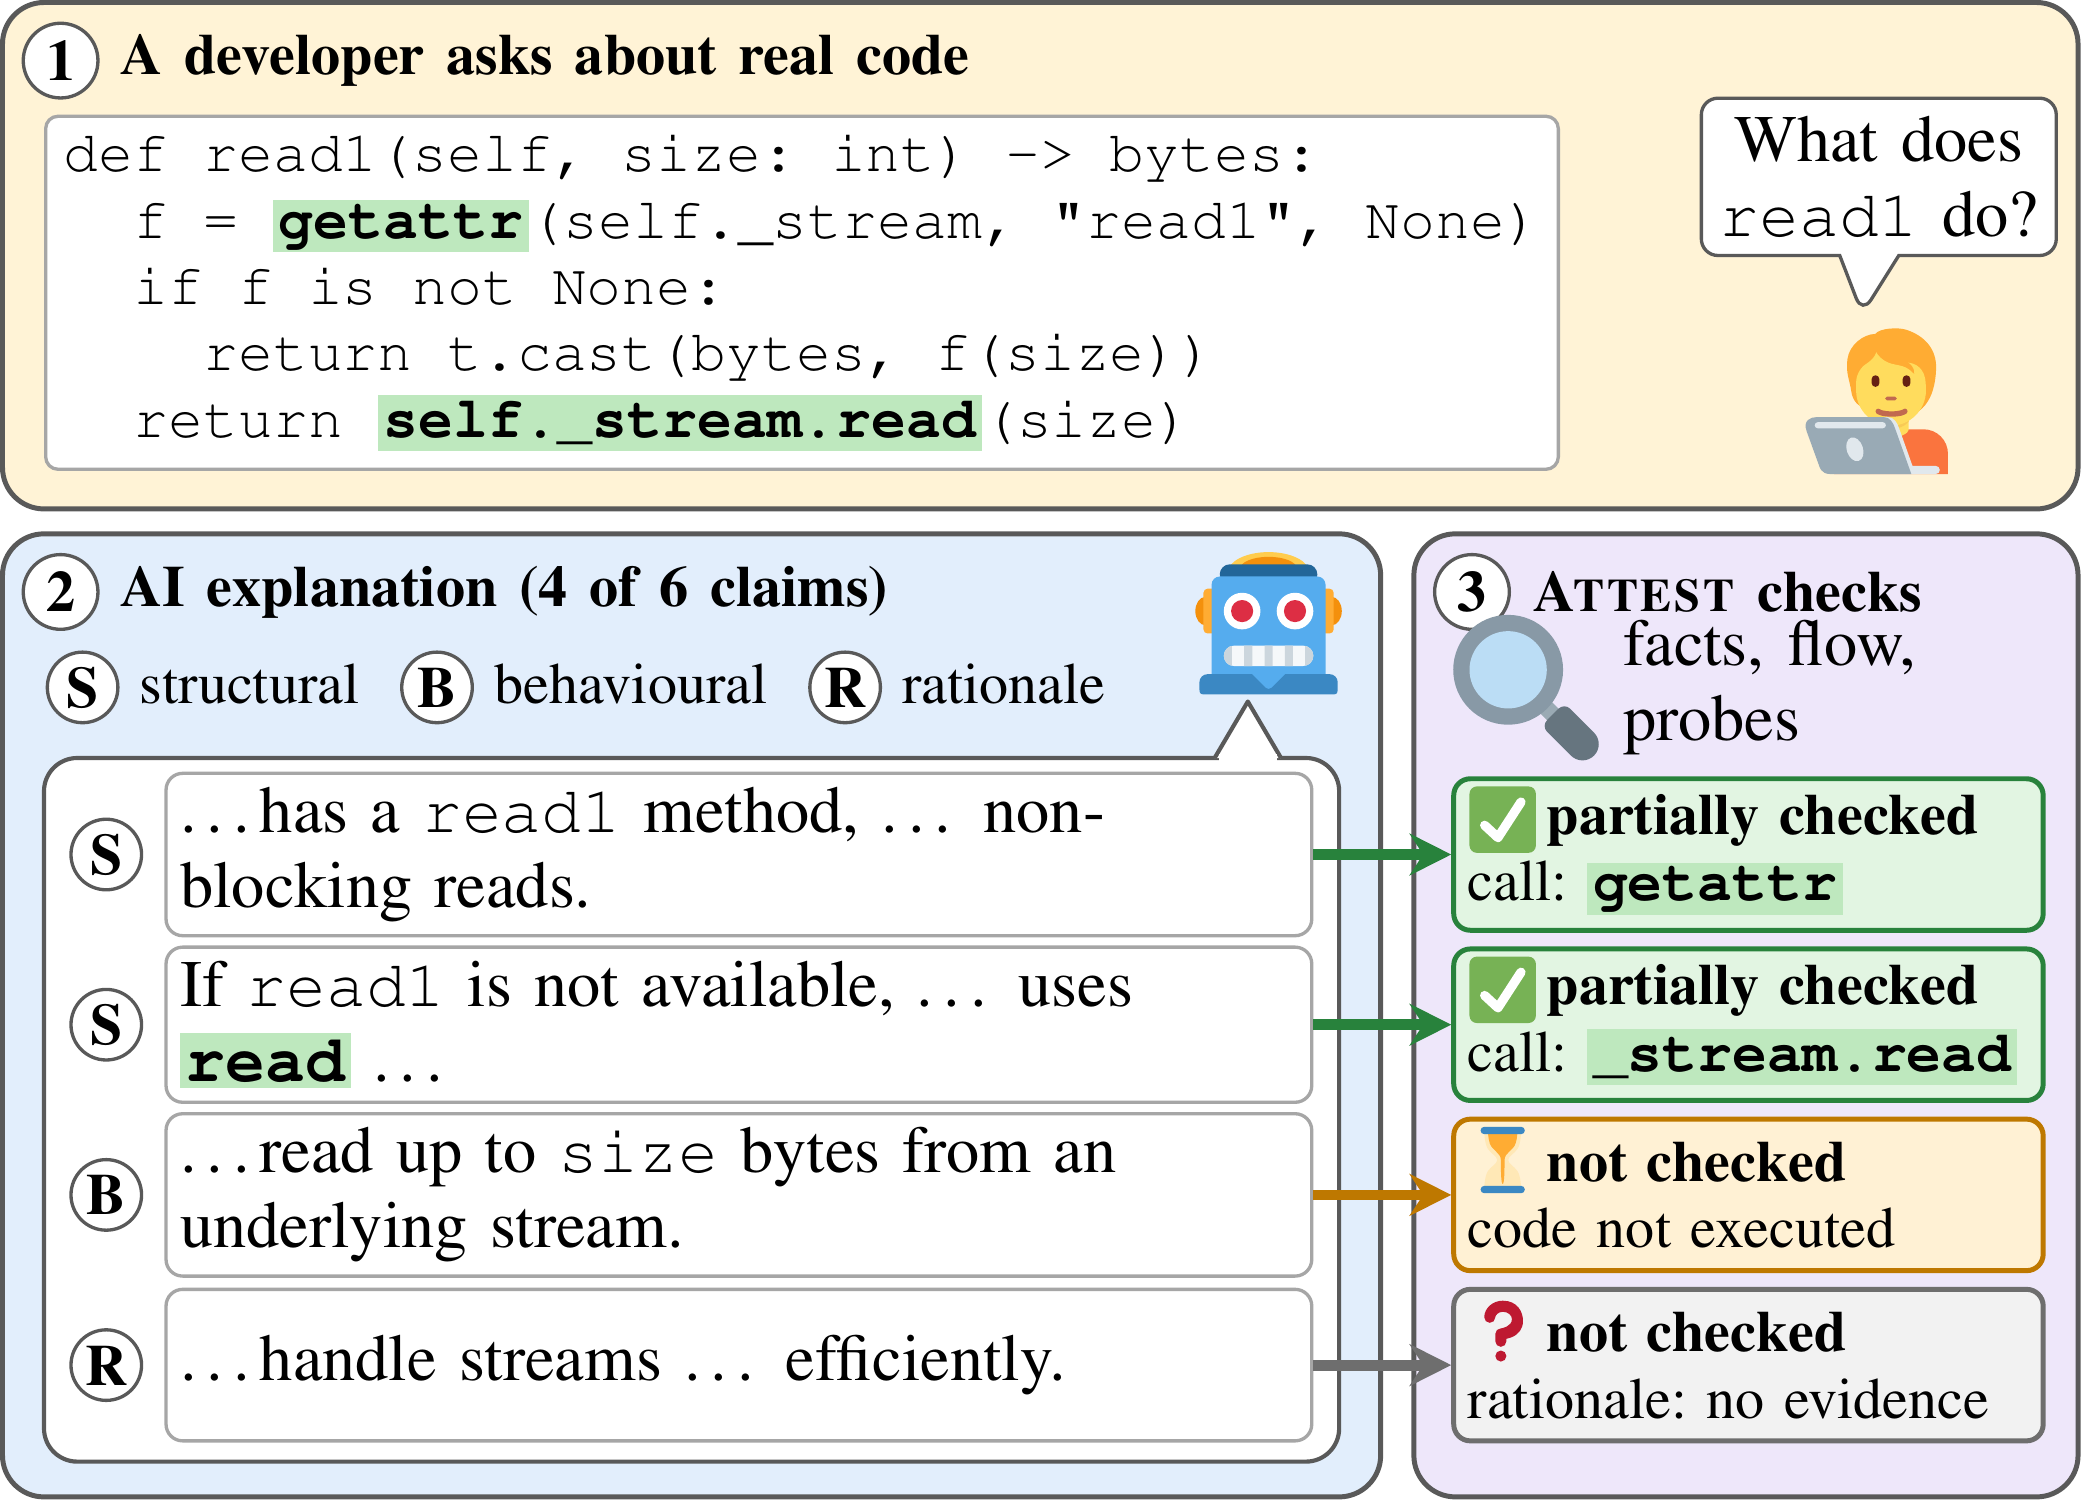
\includegraphics[width=249.664bp,height=179.925bp]{figures/figure1.png}\par\nointerlineskip
\caption{Evidence supports a specific proposition within an explanation. Four shortened claims about \texttt{read1} show supported calls alongside unassessed conditions and behaviour.}
\label{fig:example}
\end{figure}

We make that distinction explicit through evidence \emph{kind}, the source available to assess a claim, and \emph{scope}, exactly what that source supports. A \emph{slot} is an extracted field, such as a called function's name, from which we form a checkable proposition. Our \emph{slot-support contract} pairs that proposition with the surrounding content left unassessed. It makes explicit why a call-name match can coexist with an unchecked condition in the same sentence.

This focus complements the work of Sistla et al.~\cite{sistla2025verified}, our closest comparison, who verify explicit logical statements with correctness guarantees. With \attest{}, we examine code occurrences, possible value transfers and input-specific tests under an explicit scope contract. Our contribution connects these evidence kinds to sentence scope through an inspectable contract and paired diagnostics.

In an audit of our reproducible sample of 40 supported targets, an AI assistant tentatively classified 34 as partial or unrelated matches to their sentences. Our retrospective evaluation traces this mismatch through coverage and extraction. We then use simulations to prepare a study testing whether explicit evidence scope improves sentence judgments.

\section{Evidence Kinds and the Slot-Support Contract}\label{sec:approach}
Our checker extracts a target, finds evidence and reports the match alongside the original sentence. In Fig.~\ref{fig:example}, matching the \texttt{getattr} slot supports the call's occurrence, while retaining the sentence exposes its unchecked condition and behaviour.

\noindent\textbf{Evidence kinds.} What we can check depends on the claim. Structural (S) claims name code elements such as calls, while Data-flow claims describe how values reach other program points. Behavioural (B) claims describe input and output behaviour. Purpose claims concern functionality or class membership, whereas Rationale (R) claims concern design reasons or qualities such as efficiency. A second classifier separates purpose from rationale within the extractor's initial \emph{Intent} category. Figure~\ref{fig:example} uses initials for the illustrated claim kinds.

For data-flow claims, we trace possible value transfers without running the program. A \emph{may-path} says that a source could influence a destination under the analysis. It neither guarantees an executable path nor describes every execution. For behavioural claims, we use a \emph{probe}, a small executable test of a stated input and expected output. A hypothetical passing test of \texttt{read1(4)}, for example, provides evidence for that particular input. To screen probes, we check the claim's condition for applicability and require the test to reject a \emph{mutant}, a deliberately altered version of the code.

\begin{table}[t]
\centering\caption{The scope contract: read each row as the checked target and evidence (left), followed by what remains unassessed (right).}
\label{tab:contract}\footnotesize\setlength{\tabcolsep}{4pt}\renewcommand{\arraystretch}{1.05}
\begin{tabular}{@{}>{\raggedright\arraybackslash}p{.575\columnwidth}>{\raggedright\arraybackslash}p{.39\columnwidth}@{}}\toprule
\textbf{Kind: target and evidence} & \textbf{Not assessed} \\\midrule
\textbf{Structural}: syntax fact, e.g., a named call or parameter in parsed code & Conditions, whether a call runs, runtime target \\\addlinespace[2pt]
\textbf{Data-flow}: possible value-flow path between identified endpoints, respecting statement order & Executable paths, full shared-object effects, dependency on every run \\\addlinespace[2pt]
\textbf{Behavioural}: stated input/output test, condition check, rejected code mutant & Other inputs, truth of the full sentence \\\addlinespace[2pt]
\textbf{Purpose}: membership fact about the named subject, else a scoped test & Additional functionality or purpose \\\addlinespace[2pt]
\textbf{Rationale}: no evidence source in this implementation & Design reasons, which may need design records \\\bottomrule
\end{tabular}\end{table}

Table~\ref{tab:contract} sets out these boundaries: a call match leaves its execution condition unresolved, and a validated test covers limited inputs. Purpose admits narrow checks such as class membership. Rationale requires sources beyond our implementation, potentially including design records.

\noindent\textbf{Outcomes and coverage.} We report \emph{slot-supported} when the extracted target matches a fact, may-path or stated probe result within this contract. A potential rule contradiction produces a \emph{candidate refutation}, requiring semantic confirmation. Sentence truth requires a separate assessment. We use \emph{consistent} for weaker compatibility, such as control over an operation without supplying its data. Excluded execution, unsupported cases and failed probe validation receive \emph{not checked}, while \emph{outside scope} marks rationale without a corresponding evidence source.

For explanation $E$, let $C(E)$ be its extracted claims and $D(E)$ the subset receiving slot support or candidate refutation. We define the \emph{outcome share} as $\gamma=|D(E)|/|C(E)|$, where bars count claims. Two such outcomes among five claims give $\gamma=2/5$, the fraction of claims receiving either outcome. Our records retain text, slots, evidence and unassessed content, marking extractor paraphrases.

\noindent\textbf{Implementation.} Our implementation uses tree-sitter, a code parser~\cite{treesitter}, and reaching-definitions analysis, which tracks the assignments that may supply a later use. We generate probes from the signature and claim, with the function body withheld. We parse repository code without execution and run tests on the benchmark below. Known implementation limits include runtime method selection and multiple names for shared objects. Our artifact links full rules and \SuiteLim{} limitation cases in \texttt{semantic-contract.md}. Replay uses cached observations.

\section{Retrospective Findings}\label{sec:eval}
\noindent\textbf{Study setting.} We analyse \NExplanations{} saved explanations of \NFunctions{} functions: \NFuncApy{} from six Python repositories, \NFuncAjava{} from two Java repositories, and \NFuncB{} from EvalPlus, a benchmark of Python programming tasks~\cite{liu2023evalplus}. Repository functions span 5 to 45 lines at fixed revisions. We removed benchmark docstrings. We ran Qwen2.5-Coder-14B~\cite{hui2024qwencoder} and Qwen2.5-14B locally on all functions. Claude Haiku 5.5 covers three of five rounds. Fig.~\ref{fig:outcomes} abbreviates these explainers as Coder, Qwen and Haiku. Together they yield \NClaims{} extracted claims, including \RevLocalClaims{} from the two local models.

Qwen2.5-Coder extracts claims and generates probes from these explanations. Gemma2-9B and Llama3.1-8B separate Purpose from Rationale, agreeing on \RtAgree\% of cases (Cohen's chance-corrected agreement $\kappa=\RtKappa$). This measures model agreement. All rounds informed our checker development, making the results retrospective. Audits and corrected targets remain tentative assistant judgments pending independent human labels.

\subsection{Evidence coverage is concentrated in syntax and flow}
Our checker returns slot support or candidate refutation for \HoneFull\% [\HoneFullLo, \HoneFullHi] of local claims, including \HoneHeld\% [\HoneHeldLo, \HoneHeldHi] in the later three rounds. For these 95\% intervals, we resample whole functions 2,000 times, retaining their claims together. The intervals quantify function-resampling variability, excluding tuning uncertainty. Almost all of these outcomes indicate slot support (\DecTrueShare\%), but their reach varies by claim kind: outcome shares are \TypStructuralDec\% for structural claims and \TypDataflowDec\% for data flow, compared with below 1\% for behaviour.

Fig.~\ref{fig:outcomes} shows both this variation and claim composition: each bar represents one kind for one explainer, divided by outcome colour. Segment widths use the explainer's \emph{total} claims as denominator: the dark teal segment for Coder's structural claims, for instance, says that 24.6\% of all Coder claims are structural and slot-supported. The bar therefore shows this category's contribution to the full claim set. The large grey behavioural segments show where substantial content remains unchecked. Since rationale accounts for only \ResidRationale\% of local claims receiving neither outcome, our pipeline's missing support extends beyond design intent.
\begin{figure}[t]
\centering
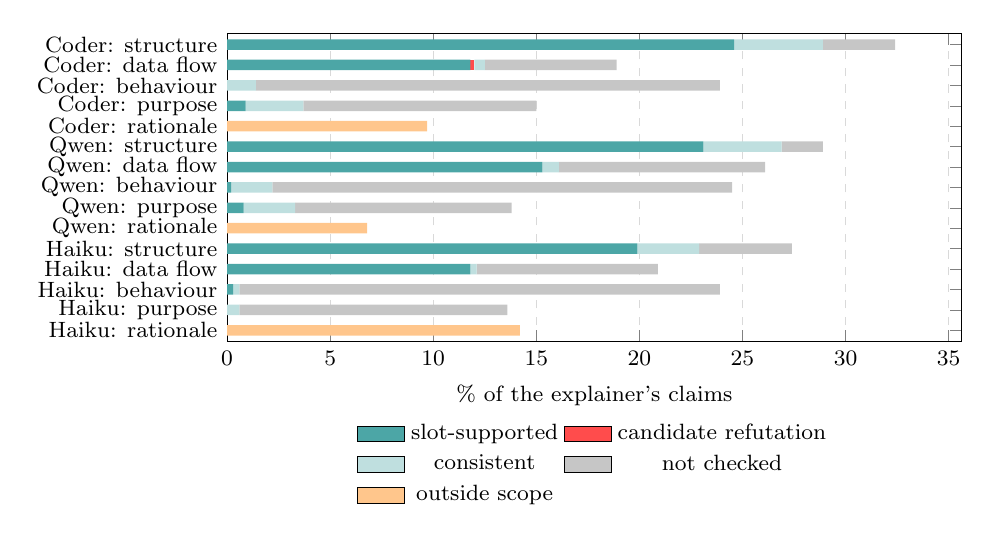
\begin{tikzpicture}
\begin{axis}[xbar stacked, width=0.90\columnwidth, height=5.5cm, bar width=3.8pt, xmin=0, xlabel={\% of the explainer's claims}, symbolic y coords={Haiku: rationale,Haiku: purpose,Haiku: behaviour,Haiku: data flow,Haiku: structure,Qwen: rationale,Qwen: purpose,Qwen: behaviour,Qwen: data flow,Qwen: structure,Coder: rationale,Coder: purpose,Coder: behaviour,Coder: data flow,Coder: structure}, ytick=data, yticklabel style={font=\footnotesize}, xticklabel style={font=\footnotesize}, label style={font=\footnotesize}, legend style={font=\footnotesize, at={(0.5,-0.23)}, anchor=north, legend columns=2, draw=none}, xmajorgrids, grid style={dashed,gray!30}, enlarge y limits=0.04]
\addplot[xbar,draw=none,fill=teal!70,area legend] coordinates {(24.6,Coder: structure) (11.8,Coder: data flow) (0.0,Coder: behaviour) (0.9,Coder: purpose) (0.0,Coder: rationale) (23.1,Qwen: structure) (15.3,Qwen: data flow) (0.2,Qwen: behaviour) (0.8,Qwen: purpose) (0.0,Qwen: rationale) (19.9,Haiku: structure) (11.8,Haiku: data flow) (0.3,Haiku: behaviour) (0.0,Haiku: purpose) (0.0,Haiku: rationale)};\addlegendentry{slot-supported}
\addplot[xbar,draw=none,fill=red!70,area legend] coordinates {(0.0,Coder: structure) (0.2,Coder: data flow) (0.0,Coder: behaviour) (0.0,Coder: purpose) (0.0,Coder: rationale) (0.0,Qwen: structure) (0.0,Qwen: data flow) (0.0,Qwen: behaviour) (0.0,Qwen: purpose) (0.0,Qwen: rationale) (0.0,Haiku: structure) (0.0,Haiku: data flow) (0.0,Haiku: behaviour) (0.0,Haiku: purpose) (0.0,Haiku: rationale)};\addlegendentry{candidate refutation}
\addplot[xbar,draw=none,fill=teal!25,area legend] coordinates {(4.3,Coder: structure) (0.5,Coder: data flow) (1.4,Coder: behaviour) (2.8,Coder: purpose) (0.0,Coder: rationale) (3.8,Qwen: structure) (0.8,Qwen: data flow) (2.0,Qwen: behaviour) (2.5,Qwen: purpose) (0.0,Qwen: rationale) (3.0,Haiku: structure) (0.3,Haiku: data flow) (0.3,Haiku: behaviour) (0.6,Haiku: purpose) (0.0,Haiku: rationale)};\addlegendentry{consistent}
\addplot[xbar,draw=none,fill=gray!45,area legend] coordinates {(3.5,Coder: structure) (6.4,Coder: data flow) (22.5,Coder: behaviour) (11.3,Coder: purpose) (0.0,Coder: rationale) (2.0,Qwen: structure) (10.0,Qwen: data flow) (22.3,Qwen: behaviour) (10.5,Qwen: purpose) (0.0,Qwen: rationale) (4.5,Haiku: structure) (8.8,Haiku: data flow) (23.3,Haiku: behaviour) (13.0,Haiku: purpose) (0.0,Haiku: rationale)};\addlegendentry{not checked}
\addplot[xbar,draw=none,fill=orange!45,area legend] coordinates {(0.0,Coder: structure) (0.0,Coder: data flow) (0.0,Coder: behaviour) (0.0,Coder: purpose) (9.7,Coder: rationale) (0.0,Qwen: structure) (0.0,Qwen: data flow) (0.0,Qwen: behaviour) (0.0,Qwen: purpose) (6.8,Qwen: rationale) (0.0,Haiku: structure) (0.0,Haiku: data flow) (0.0,Haiku: behaviour) (0.0,Haiku: purpose) (14.2,Haiku: rationale)};\addlegendentry{outside scope}
\end{axis}
\end{tikzpicture}
\caption{Claim composition and outcomes. Coder = Qwen2.5-Coder-14B, Qwen = Qwen2.5-14B and Haiku = Claude Haiku 5.5. Segment widths show each category's share of the explainer's total claims.}
\label{fig:outcomes}
\end{figure}


\subsection{Supported slots often leave sentence content unassessed}
We assess sentence-level alignment using a reproducible, seeded random sample of 40 of the \RevSupported{} local slot-supported verdicts. The assistant classified six as \emph{full-scope}, meaning that the evidence covered the sentence's assertions, 33 as asserting more than their slots and one as unrelated. Multiplying the supported share by the audited full-scope fraction gives our estimate across all local claims: $(\RevSupported/\RevLocalClaims)(6/40)=\RevFullShare\%$. Inverting the hypergeometric distribution for sampling without replacement gives a 95\% finite-population interval [\RevFullLo, \RevFullHi]. This interval conditions on our corpus and tentative labels. Sentence truth still requires a separate assessment.

\begin{table}[t]\centering\caption{Policy coverage among all 822 local claims. Audit mismatch counts partial/unrelated judgments over audited accepted claims. Sentence truth requires separate assessment.}\label{tab:risk}\footnotesize\begin{tabular}{@{}lrr@{}}\toprule Policy & Coverage \% & Audit mismatch \\\midrule
Exact syntax baseline & 18.9 & 20/20 \\
Exact structural support & 23.5 & 23/27 \\
Structural + flow support & 37.3 & 34/39 \\
All supported outcomes & 38.3 & 34/40 \\\bottomrule\end{tabular}\end{table}

These mismatches led us to compare four fixed display \emph{policies}, each selecting which results to show (Table~\ref{tab:risk}). Our syntax baseline directly matches extracted call or parameter names, whereas the other policies accept supported outcomes from exact structural rules, structural plus data-flow rules, or all rules. Coverage divides accepted claims by all \RevLocalClaims{} local claims. ``Audit mismatch'' divides partial/unrelated judgments by audited accepted claims. Thus displaying all supported outcomes covers 38.3\%, with 34 mismatches among 40 audited cases. The baseline accepts less, yet all 20 of its audited cases mismatch. These counts describe scope mismatch. Sentence truth and slot correctness require separate validation. Our bounds allow unaudited labels to take either value.

\subsection{Extracted representations change checker outcomes}
\begin{table}[t]
\centering\caption{Planted pairs: original and altered statements. Unmatched counts failed extractions over both twins. Candidate refutation and slot support count altered twins only. Construction (nominal) truth labels are unvalidated.}
\label{tab:planted}\footnotesize\setlength{\tabcolsep}{3pt}
\begin{tabular}{@{}lrrrr@{}}\toprule
Pair set & Pairs & Unmatched & \shortstack{Candidate\\refutation} & \shortstack{Slot\\support} \\\midrule
All frozen (nominal) & 151 & 26/302 & 44/151 & 33/151 \\
No known label errors & 148 & 26/296 & 43/148 & 31/148 \\
Original supported & 116 & 24/232 & 42/116 & 28/116 \\
\bottomrule\end{tabular}\end{table}

To investigate where mismatches begin, we use \emph{planted pairs}: an original statement and a deliberately altered counterpart, whose members we call \emph{twins}. Their \emph{nominal} true/false labels inherit construction and engine judgments and await independent validation. We retain all 151 pairs in Table~\ref{tab:planted}. Removing three assistant-identified label-error pairs gives its second row. Further excluding 32 pairs whose originals no longer receive slot support leaves the 116 pairs in its last row. Targeted assistant audits cover 31 pairs.

In the complete set, extraction failed to match 26 of 302 twins, while 44 of 151 altered twins received candidate refutation and 33 received slot support. The different denominators matter: ``Unmatched'' counts both twins, but refutation and support count altered twins only. These pair sets expose selection effects without resolving nominal-label uncertainty.

Holding the checker and facts fixed, we next change only the extracted targets. An assistant prepared and froze corrected targets for all \RevAblPairs{} structural/data-flow pairs (\RevAblTwins{} twins), retaining sentences, conditions and receivers, the objects on which methods are called. The annotations mark \RevAblUnrep{} twins as unrepresentable by one faithful target. These corrections start from the original slots, so they are neither blinded nor independently validated reference (``gold'') annotations.

With those corrected targets, Slot-supported outcomes on nominal altered twins fall from \RevAblBefore{} to \RevAblAfter{}. The original extraction leaves \RevAblLost{} twins unmatched. These transitions measure representation sensitivity. Residual support may concern another subclaim or reflect a wrong label or checker error. In the five remaining cases, assistant inspection found confused name/role matches, unchecked conditions and confusion between converting a value and passing it along. We retain each twin's before/after outcomes and examples in the artifact.

How often false claims occur also matters. Refutation \emph{precision}, the fraction of candidate refutations assigned a nominal false label, is \RevPrecHalf\% in our selected-pair sensitivity calculation when 50\% of claims are assumed false. It falls to \RevPrecOne\%, \RevPrecFive\% and \RevPrecTen\% at 1\%, 5\% and 10\%, respectively: when false claims are rare, contradictions issued on true claims can dominate the alerts. These calculations describe assumed prevalence scenarios. Deployment estimates would require representative data. Our current corpus contains one candidate refutation, judged correct by the assistant after rules were revised using this corpus. Our artifact includes function-resampling intervals and the 25\% scenario.

\section{Implications and a Scoped-Badge Study}\label{sec:agenda}
\noindent\textbf{Reading a badge.} We translate the scope contract into a proposed display such as ``call found, non-blocking behaviour unassessed'' for the first sentence in Fig.~\ref{fig:example}. Our planned study tests its effect on sentence judgments, motivated by evidence that automation cues can encourage misuse~\cite{parasuraman1997automation,bucinca2021trust}. We distinguish three properties: coverage counts the targets receiving a result, correctness concerns whether that result is right, and sentence sufficiency concerns whether its evidence covers the whole assertion. Improving one need not improve the others.

A false sentence with a valid subclaim makes this distinction concrete. Consider the hypothetical ``This calls \texttt{read} and never waits,'' when the call exists but can wait. Highlighting the call supplies valid evidence for the subclaim, yet leaves the whole sentence unjustified. This case guides our planned study.

\noindent\textbf{Primary comparison.} We will compare scoped badges, which display the supported proposition and unassessed content, with generic ``checked'' badges on these false partial-support sentences. Our primary outcome is correct rejection of the whole sentence. A third condition presents prose with code links. All conditions provide identical code/evidence access.

Before recruitment, we require two independent humans to validate sentence truth, evidence validity and evidence sufficiency separately. Each participant will see 24 distinct items, eight per condition. We use balanced Latin-square assignment to rotate item blocks across interfaces without repeating an item within a participant. Each condition has four true and four false sentences. The false items comprise two valid partial-support, one misleading-evidence and one no-evidence item. Alongside evidence comprehension, we will record clicks, time, confidence accuracy (Brier score: squared error of a probability judgment) and judgments of nearby unbadged statements~\cite{pennycook2020impliedtruth}. These secondary measures include clicks, which alone do not establish comprehension. Our artifact details allocation, ethics, consent, debriefing and registration requirements.

% Balance the final main-text page, leaving the references on their own page.
\balance
\noindent\textbf{Design sensitivity.} Our planned logistic mixed model estimates correct-rejection probability with participant and item baseline variation (crossed random intercepts). Interface condition, evidence category and their interaction let the badge effect vary by evidence kind. Our primary test checks for either an increase or decrease within partial-support items at the 5\% significance level.

We fitted this model with the R package \texttt{lme4} to 60,000 simulated datasets: five participant counts, four target odds ratios and three levels of participant/item variation, with 1,000 repetitions per setting. For rejection probability $p$, odds are $p/(1-p)$. An odds ratio (OR) of 1.65 multiplies them by 1.65 with participant/item effects fixed. Power, the fraction of simulations detecting that effect, is \RevPowerSmall{} with 36 participants and \RevPowerLargest{} with 216. With no badge effect (OR 1), false-positive rates are \RevNullRange{}. Monte Carlo standard error, uncertainty from finite repetitions, is at most 0.016. We count fits that fail to settle on stable estimates (converge) as non-detections and report them separately from singular fits, where estimated participant or item variation collapses to zero.

Our simulations hold badge effects constant across participants and items and exclude learning and dropout. We will set the recruitment target after agreeing on a minimum meaningful effect. Participant outcomes remain pending. The next evaluation phase requires independent labels, validated reference slots and a fresh corpus.

\section{Related Work}
\noindent\textbf{Describing explanation content.} Pennington's program models separate operations, control flow, data flow and function~\cite{pennington1987}, while comment taxonomies distinguish what, why, how-it-is-done, property and usage~\cite{chen2021commentcategory}. Our grouping of claim kinds adds the evidence kind and scope available to assess such content. For generated summaries, ETF, an entity-tracing framework, follows names in summaries~\cite{etf2025}, while ReFEree scores segments against dependency context~\cite{referee2026}. Khatib et al.\ show that summaries can miss behaviour-changing mutations~\cite{khatib2026mutation}. We examine where a checked proposition leaves its surrounding sentence unresolved.

\noindent\textbf{Checking claims against code.} @tComment tests null-related Javadoc properties~\cite{tan2012tcomment}, and Jdoctor and C2S translate comments into specifications~\cite{blasi2018jdoctor,zhai2020c2s}. nl2postcond generates postconditions, properties expected to hold after a function returns~\cite{endres2024nl2postcond}. Sistla et al.\ soundly verify formalised explanation claims, validating 18 of 88 valid explanations with one formalisation pass and 36 with five~\cite{sistla2025verified}. Our corrected-target diagnostic examines representation sensitivity in a heuristic checker. Other approaches offer complementary evidence: EVIDENT validates generated analysis programs~\cite{evident2026}, traces record program steps that can ground rationales~\cite{thakur2025verifiablecot}, and work on checkable justifications~\cite{xu2025justifications} and code-location links~\cite{arafat2025citation} helps readers inspect an answer's basis.

\noindent\textbf{Interpreting evidence cues.} Readers' interpretation of automation shapes how they use evidence~\cite{lee2004trust}. Explanations can encourage over-reliance when verification is costly~\cite{vasconcelos2023explanations}. Generative AI also places demands on monitoring and checking one's understanding~\cite{tankelevitch2024metacognitive}. Trust changes with experience of coding assistants~\cite{trustdynamics2025}, and models' reported confidence poorly matches their accuracy~\cite{spiess2025calibration}. These findings motivate our planned comparison of evidence displays while holding the evidence fixed. For design rationale, they also connect to the longer-term problem of preserving intent~\cite{storey2026intentdebt}.

\section{Conclusion}
We provide an explicit contract for connecting extracted code facts to explanation sentences. The tentative assistant audit identifies frequent scope mismatches, and our paired diagnostics trace outcome changes to representation. Together, these results make evidence scope a concrete evaluation target. The next phase combines independent label validation with the planned reader study to test whether displaying that scope improves developers' judgments.

\smallskip\noindent\textbf{AI use and data availability.} We use language models as experimental subjects. An AI assistant wrote code, performed the tentative audits and slot corrections, and revised the text. Independent validation of semantic labels and reference slots remains pending, as do participant outcomes. Our frozen package supplies code, cached inputs, annotations, specifications and results. Run \texttt{make replay} in its artifact directory. This manuscript revises their presentation. The anonymous artifact package is available at \ArtifactLink.


\clearpage
\nobalance
\bibliographystyle{IEEEtran}
\bibliography{references}
\end{document}
